\subsection{\href{http://www.softron.biz/}{Softron}}
   \hypertarget{subsec:softron}
   La empresa Softron S.A provee soluciones al mercado mayorista de proveedores de energía, instalando medidores de consumo y ofreciendo el servicio de monitoreo remoto. \\
   Para dicha empresa se desarrollaron placas de integración entre SBC, computadoras en una placa, y periféricos como, salidas de relé, entradas IO's, fuentes de alimentación, soporte para modulo GSM y dual SIM, entre otras opciones. Se pueden ver algunas fotos de la placa desarrollada en la figura \ref{fig:softron1} para la cual se realizaron varios prototipos y se genero toda la documentación de fabricación en volumen. \\
   Por otra parte también se diseñaron dispositivos inalámbricos para monitoreo de temperatura usando redes Zigbee en modo mesh, se pueden ver algunas fotos de los equipos fabricados en la figura \ref{fig:softron1}. \\
   \begin{figure}
      \begin{center}
         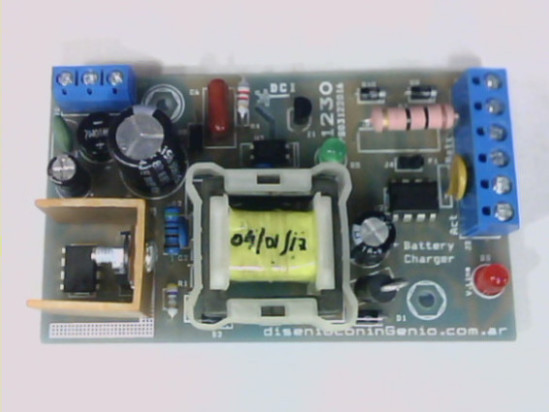
\includegraphics[width=0.24\textwidth]{softron1.jpg}
         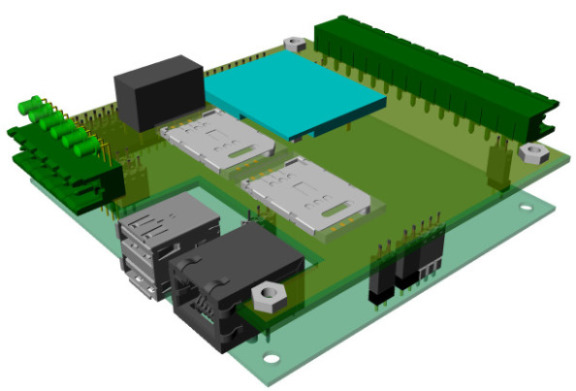
\includegraphics[width=0.24\textwidth]{softron2.jpg}
         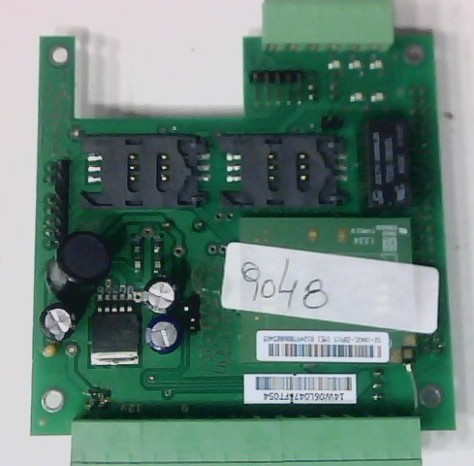
\includegraphics[width=0.24\textwidth]{softron3.jpg}
         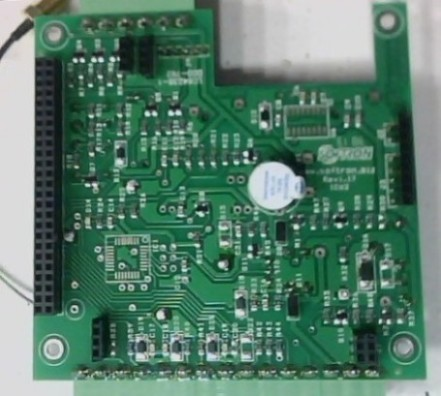
\includegraphics[width=0.24\textwidth]{softron4.jpg}
      \end{center}
      \caption{Placa de integración entre una SBC y una amplia gama de periféricos, modulo GSM, fuente de alimentación y conectores.}
      \label{fig:softron1}
   \end{figure}
